\section{Synthetic ruptures}
\label{sec:synthetic}

\subsection{Set-up}
The synthetic pairs (Appendix~\ref{app:synthetic}) put a vertical strike-slip rupture and an ionosphere into a 96\,km
scene. Each 40\,m pixel of each band is drawn from the complex Wishart distribution of its looks, with a coherence
that combines a far-field value, a damage zone along the trace and the fringe-rate loss. The pixels are summed into
240\,m cells exactly as GSLC pixels are. Every estimator then runs on the same cells, with the same fault-zone
exclusion (2\,km, unless stated), the same filter (the v6 settings of Section~\ref{sec:estimator}) and the same
main-band unwrapping (the oracle: the truth's integers). The estimators are:
\begin{description}
  \item[reordered (ours)] Eq.~\eqref{eq:ours}, with $r$ unwrapped as in Section~\ref{sec:estimator};
  \item[reformulated, same unwrapper] Eq.~\eqref{eq:reform}, with $\Delta$ unwrapped by \emph{our} unwrapper. This
        is the controlled comparison: it differs from ours only in when $(\Delta f/\fA)\phiA$ is subtracted;
  \item[reformulated (SNAPHU)] Eq.~\eqref{eq:reform} with $\Delta$ unwrapped by SNAPHU on the cells, as ISCE3
        unwraps it;
  \item[reformulated, wrapped] Eq.~\eqref{eq:reform} with $\Delta$ taken about its circular mean, the
        ``lowest ambiguity'' of \citet{wegmuller2018reformulating};
  \item[reformulated + ISCE3 corrections] the GUNW recipe: SNAPHU, then ISCE3's two correction passes
        (Section~\ref{sec:corrections}, Appendix~\ref{app:isce3});
  \item[two-band] Eq.~\eqref{eq:twoband} with $\phiB$ unwrapped by SNAPHU, bare, with ISCE2's relative correction,
        or with ISCE3's two passes.
\end{description}
Errors are the filtered screen minus the true ionosphere, less their median beyond 20\,km. The leak is the slope of
the error's 15\,km high-pass on the deformation's, within 10\,km of the trace. That is the statistic of the GUNW
comparisons in Section~\ref{sec:nisar}, with the truth in place of the data. Each case has three noise realizations,
and the spread between them is small next to the differences between estimators.

\subsection{Results}
Tables~\ref{tab:synthetic} and \ref{tab:robust} and Figures~\ref{fig:maps}--\ref{fig:sweep} summarise them; all
numbers are in mm of LOS ($\lambda_A/4\pi = 19.3$\,mm per radian). Four findings stand out.

\paragraph{With nothing to unwrap through, the forms agree.} On a rupture that ends inside the scene, with the fault
zone excluded, every estimator without corrections returns the same screen as ours at peak slips up to 4\,m. This
holds for the two-band form too, with the side band unwrapped on its own. The unwrapper can integrate around the
rupture's ends, and outside the excluded zone the deformation is smooth enough for SNAPHU at 216 side-band looks per
cell. Their error 2--5\,km from the trace is 8.5--8.8\,mm at every slip and 8.4\,mm at zero slip, 1.9\,mm beyond
20\,km. It is the filter's, not the rupture's: its fill of the excluded zone (18\,mm rms inside it) and its weighted
mean's lag across the damage zone (Section~\ref{sec:nearfield}). On the same scene without slip the error near the
trace is the same to a millimetre. Our estimate's apparent slope on the
deformation falls as the slip grows ($-0.012$ at 1\,m, $-0.004$ at 4\,m, $-0.003$ at 6\,m). That is a fixed residual
projected onto a growing pattern, not a copy of it.

\paragraph{The correction passes leak at every slip.} ISCE3's two passes, applied to the reformulated or the two-band
form, are the only estimators that leak on the benign geometry. They copy $-0.045$ to $-0.048$ of the high-passed
deformation (mean over seeds) at every peak slip from 1 to 6\,m, a fixed fraction, so the absolute error grows with the slip. At
2--5\,km from the trace it is 14\,mm at 1\,m of slip, 25\,mm at 2\,m, 47\,mm at 4\,m and 68\,mm at 6\,m. At 4\,m the
passes move a main-band cycle at 3\% of the cells used, in bands along the trace where the deformation's curvature
takes it more than $\pi$ from its 2\,km low-pass (Fig.~\ref{fig:maps}). The screen then steps 97\,mm across the trace,
with the sign of the deformation reversed. Without the fault-zone exclusion, which ISCE3 does not apply, the passes
move cycles at 9.5\% of the cells and the leak grows to $-0.062$ (90\,mm at 2--5\,km, a 185\,mm step).

\paragraph{A rupture that splits the scene breaks every form that unwraps deformation.} When the rupture runs through
the scene, its two sides meet only across the fault zone, and an unwrapper must choose the cross-fault integer
without data.
\begin{itemize}
  \item The two-band form's side band carries the whole step. Its error 2--5\,km from the trace is 2.1\,m at 1\,m of
        slip and 9\,m at 4\,m. ISCE2's relative correction brings that down to 0.4--3\,m, and ISCE3's passes do not
        help.
  \item The reformulated form's $\Delta$ carries 4.4\% of the step, and fails once that exceeds about $\pi$. With our
        unwrapper, which bridges the gap by the shortest arc, it fails at 4\,m of slip. With SNAPHU it fails at 6\,m,
        and so does the GUNW recipe. Taken as wrapped, it fails at 6\,m, and at 4\,m when a coastline removes most of
        the north side. Each failure is one cycle of $\Delta$ between the sides: 73\,rad, or 1.4\,m of LOS
        (Fig.~\ref{fig:profiles}). After a median is removed over both sides' far field, that reads as $\pm$0.7\,m.
  \item The reordered form's error stays at its zero-slip level in every case: 8.2--8.6\,mm at 2--5\,km and 2\,mm
        beyond 20\,km.
\end{itemize}
The controlled pair, ``reformulated, same unwrapper'' against ours, isolates the cause. The two differ only in when
$(\Delta f/\fA)\phiA$ is subtracted, and only the reordered one survives. Without the exclusion, ours does better
still inside the fault zone (8.6\,mm rms within 2\,km, where it is no longer filled), and SNAPHU's $\Delta$ again
fails at 6\,m.

\paragraph{Low coherence, coastlines and patchy decorrelation change little} (Table~\ref{tab:robust}). Reducing the
far-field coherence to 0.35, removing the north side beyond 2\,km on half the rupture, or decorrelating a quarter of
the ground within 10\,km of the trace in 0.5\,km blobs leaves the pattern above unchanged. Ours stays at 8--12\,mm,
the correction passes leak $-0.031$ to $-0.046$, and the forms that unwrap deformation fail as on the plain
through-going rupture. What decides the outcome is geometry: whether the unwrapped field has to cross the rupture.

\paragraph{Band co-location and the main band's integers.} Sampling the side band 3, 9 or 20\,m further down range
changes the error at 2--5\,km by 0.03, 0.3 and 1.2\,mm in this geometry, the same for all forms
(Section~\ref{sec:colocation}). Moving the main band's south side by one cycle, as a wrong tie of a cut-off block
would, moves the raw estimate there by exactly 3.21\,rad (62\,mm) in ours and every reformulated form, and by
76.2\,rad in the two-band form (Table~\ref{tab:integers}). Far from the trace that is a constant per block. Near it the
filter mixes the blocks across the excluded zone: relative to the block's own offset, the screen is 23\,mm high within
2\,km north of the trace and 19\,mm low within 2\,km south, a 42\,mm fake step. D141's measured 5\,cm per cycle
(Section~\ref{sec:tie}) is the same effect.

\begin{table}[t]
\centering
\caption{Synthetic results at 4\,m peak slip, mean of three noise realizations: error rms in distance bands from
the trace (mm of LOS), the leak (slope of the error's 15\,km high-pass on the deformation's, within 10\,km), and the
error's step from 2--4\,km south to 2--4\,km north (mm).}
\label{tab:synthetic}
\scriptsize
\setlength{\tabcolsep}{4pt}
\begin{tabular}{llrrrrrr}
\toprule
case & estimator & 0--2\,km & 2--5\,km & 5--10\,km & $>$20\,km & leak & step \\
 & & \multicolumn{4}{c}{error rms (mm LOS)} & & (mm) \\
\midrule
finite rupture & reordered (ours) & 18.5 & 8.8 & 1.9 & 1.9 & -0.004 & 8.2 \\
 & reformulated, same unwrapper & 18.5 & 8.8 & 1.9 & 1.9 & -0.004 & 8.2 \\
 & reformulated (SNAPHU) & 18.5 & 8.8 & 1.9 & 1.9 & -0.004 & 8.2 \\
 & reformulated, wrapped & 18.5 & 8.8 & 1.9 & 1.9 & -0.004 & 8.2 \\
 & reformulated + ISCE3 corrections & 41.4 & 46.5 & 14.2 & 1.9 & -0.047 & 96.6 \\
 & two-band (SNAPHU) & 18.5 & 8.8 & 1.9 & 1.9 & -0.004 & 8.2 \\
 & two-band + ISCE2 correction & 18.5 & 8.8 & 1.9 & 1.9 & -0.004 & 8.2 \\
 & two-band + ISCE3 corrections & 39.9 & 47.1 & 14.7 & 1.9 & -0.048 & 98.1 \\
\midrule
through-going & reordered (ours) & 16.9 & 8.3 & 1.8 & 2.0 & -0.003 & 8.3 \\
 & reformulated, same unwrapper & 213.8 & 539.8 & 698.1 & 703.1 & 0.444 & -975.4 \\
 & reformulated (SNAPHU) & 16.9 & 8.3 & 1.8 & 2.0 & -0.003 & 8.3 \\
 & reformulated, wrapped & 17.5 & 8.5 & 1.8 & 2.0 & -0.002 & 7.5 \\
 & reformulated + ISCE3 corrections & 44.8 & 57.4 & 19.7 & 2.0 & -0.043 & 119.4 \\
 & two-band (SNAPHU) & 3477.2 & 9032.0 & 1.2e4 & 1.2e4 & 7.431 & -1.6e4 \\
 & two-band + ISCE2 correction & 1083.0 & 1977.9 & 3318.5 & 1.3e4 & 0.391 & -3168.5 \\
 & two-band + ISCE3 corrections & 2893.0 & 8127.5 & 1.2e4 & 1.2e4 & 6.726 & -1.4e4 \\
\midrule
through-going, no exclusion & reordered (ours) & 8.6 & 7.1 & 1.8 & 2.0 & -0.005 & 14.4 \\
 & reformulated, same unwrapper & 333.6 & 630.9 & 701.4 & 703.1 & 0.512 & -1211.9 \\
 & reformulated (SNAPHU) & 8.6 & 7.1 & 1.8 & 2.0 & -0.005 & 14.4 \\
 & reformulated, wrapped & 35.3 & 22.3 & 3.6 & 2.0 & 0.002 & 3.6 \\
 & reformulated + ISCE3 corrections & 100.6 & 89.5 & 21.1 & 2.0 & -0.062 & 184.7 \\
 & two-band (SNAPHU) & 6467.0 & 1.2e4 & 1.3e4 & 1.3e4 & 9.794 & -2.3e4 \\
 & two-band + ISCE2 correction & 1367.3 & 2321.7 & 3672.5 & 1.4e4 & 0.553 & -3970.5 \\
 & two-band + ISCE3 corrections & 5742.0 & 1.1e4 & 1.3e4 & 1.3e4 & 9.207 & -2.1e4 \\
\bottomrule
\end{tabular}

\end{table}

\begin{table}[t]
\centering
\caption{As Table~\ref{tab:synthetic}, through-going rupture at 4\,m, for harder data: far-field coherence 0.35;
water north of the trace's eastern half beyond 2\,km; a quarter of the ground within 10\,km of the trace decorrelated
in 0.5\,km blobs.}
\label{tab:robust}
\scriptsize
\setlength{\tabcolsep}{4pt}
\begin{tabular}{llrrrrrr}
\toprule
case & estimator & 0--2\,km & 2--5\,km & 5--10\,km & $>$20\,km & leak & step \\
 & & \multicolumn{4}{c}{error rms (mm LOS)} & & (mm) \\
\midrule
coherence 0.35 & reordered (ours) & 16.6 & 8.2 & 2.0 & 2.3 & -0.002 & 5.6 \\
 & reformulated, same unwrapper & 222.7 & 547.1 & 698.1 & 703.1 & 0.451 & -996.9 \\
 & reformulated (SNAPHU) & 16.6 & 8.2 & 2.0 & 2.3 & -0.002 & 5.6 \\
 & reformulated + ISCE3 corrections & 45.6 & 60.6 & 20.7 & 2.3 & -0.046 & 125.8 \\
 & two-band (SNAPHU) & 3590.6 & 9127.6 & 1.2e4 & 1.2e4 & 7.522 & -1.6e4 \\
\midrule
coast & reordered (ours) & 20.2 & 8.1 & 2.2 & 2.1 & -0.004 & 3.2 \\
 & reformulated, same unwrapper & 524.8 & 722.2 & 815.9 & 799.7 & 0.315 & -1049.0 \\
 & reformulated (SNAPHU) & 20.2 & 8.1 & 2.2 & 2.1 & -0.004 & 3.2 \\
 & reformulated + ISCE3 corrections & 41.6 & 52.5 & 18.0 & 2.1 & -0.031 & 103.8 \\
 & two-band (SNAPHU) & 7620.0 & 1.0e4 & 1.2e4 & 1.2e4 & 4.568 & -1.5e4 \\
\midrule
patchy decorrelation & reordered (ours) & 20.3 & 11.3 & 4.9 & 1.9 & -0.003 & 7.9 \\
 & reformulated, same unwrapper & 192.9 & 486.0 & 657.7 & 703.0 & 0.394 & -868.6 \\
 & reformulated (SNAPHU) & 20.3 & 11.3 & 4.9 & 1.9 & -0.003 & 7.9 \\
 & reformulated + ISCE3 corrections & 42.1 & 50.2 & 18.5 & 1.9 & -0.037 & 99.7 \\
 & two-band (SNAPHU) & 3120.1 & 7784.2 & 1.1e4 & 1.1e4 & 6.324 & -1.4e4 \\
\bottomrule
\end{tabular}

\end{table}

\begin{figure}[t]
\centering
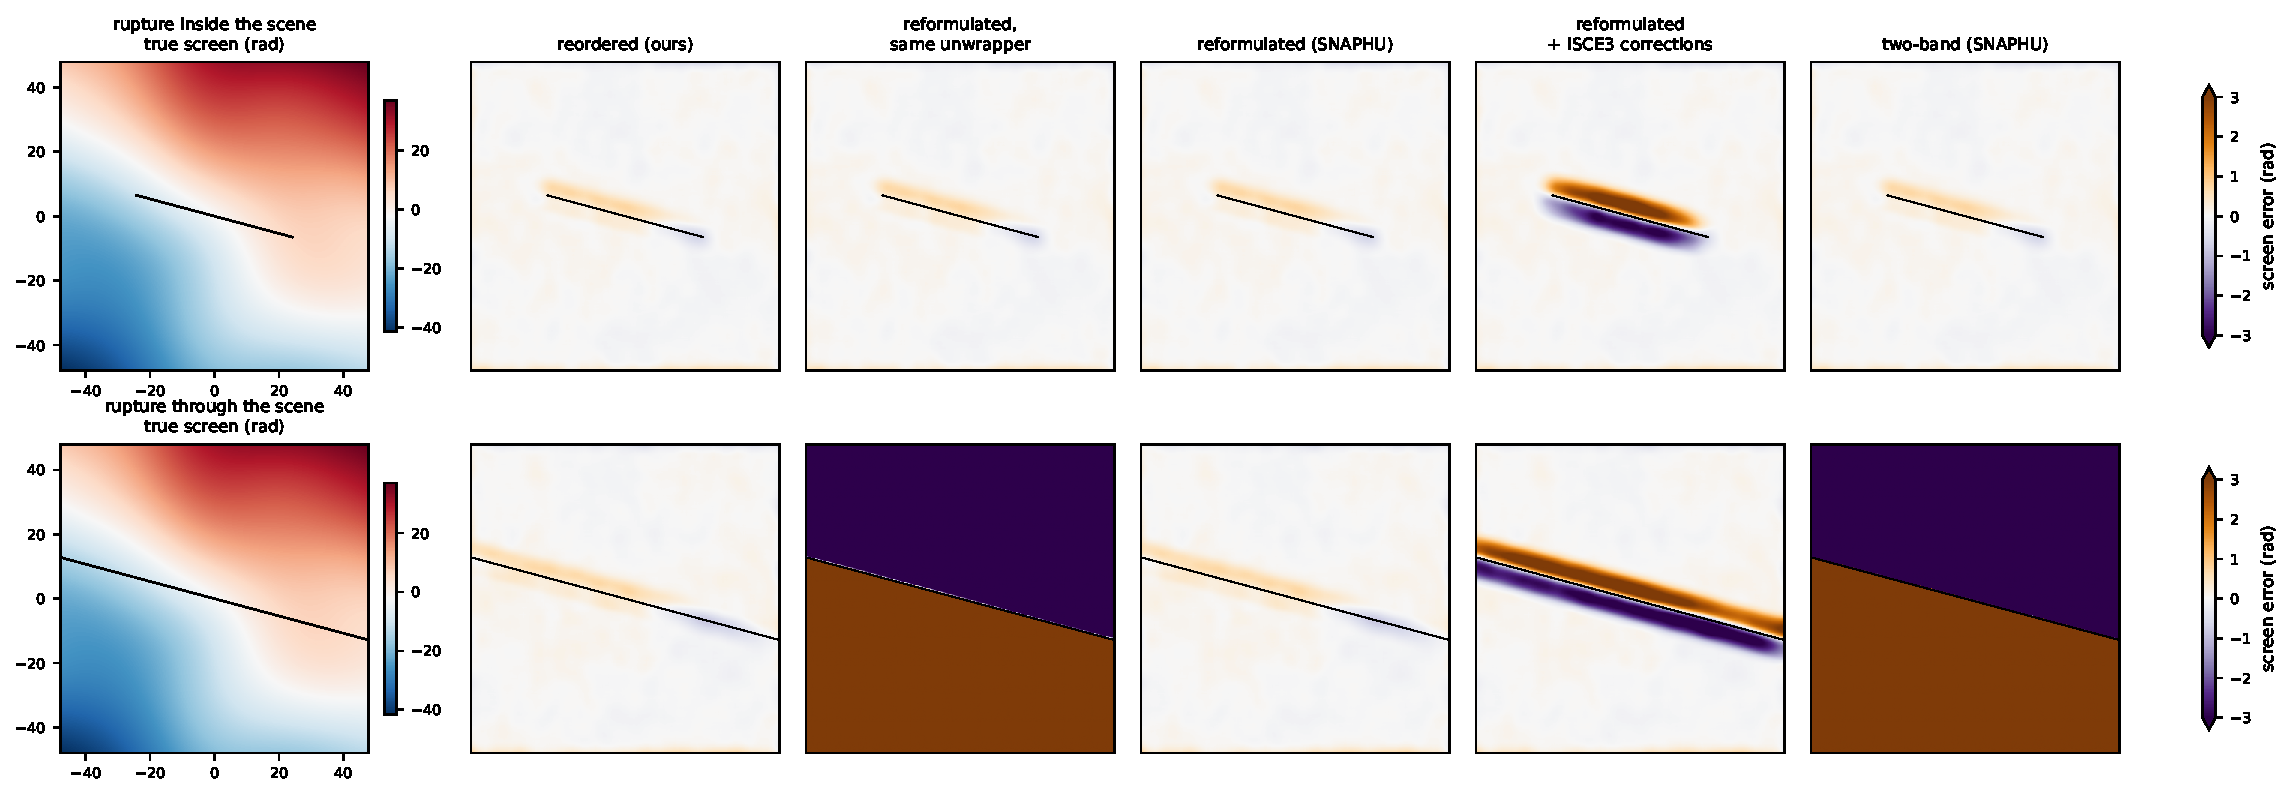
\includegraphics[width=\textwidth]{figures/fig_maps}
\caption{Screen errors (rad) on the two example scenes, 4\,m peak slip, one noise realization, for five of the eight
estimators. Top: a 50\,km rupture inside the scene. Bottom: a 160\,km rupture through it. Left: the true ionosphere.}
\label{fig:maps}
\end{figure}

\begin{figure}[t]
\centering
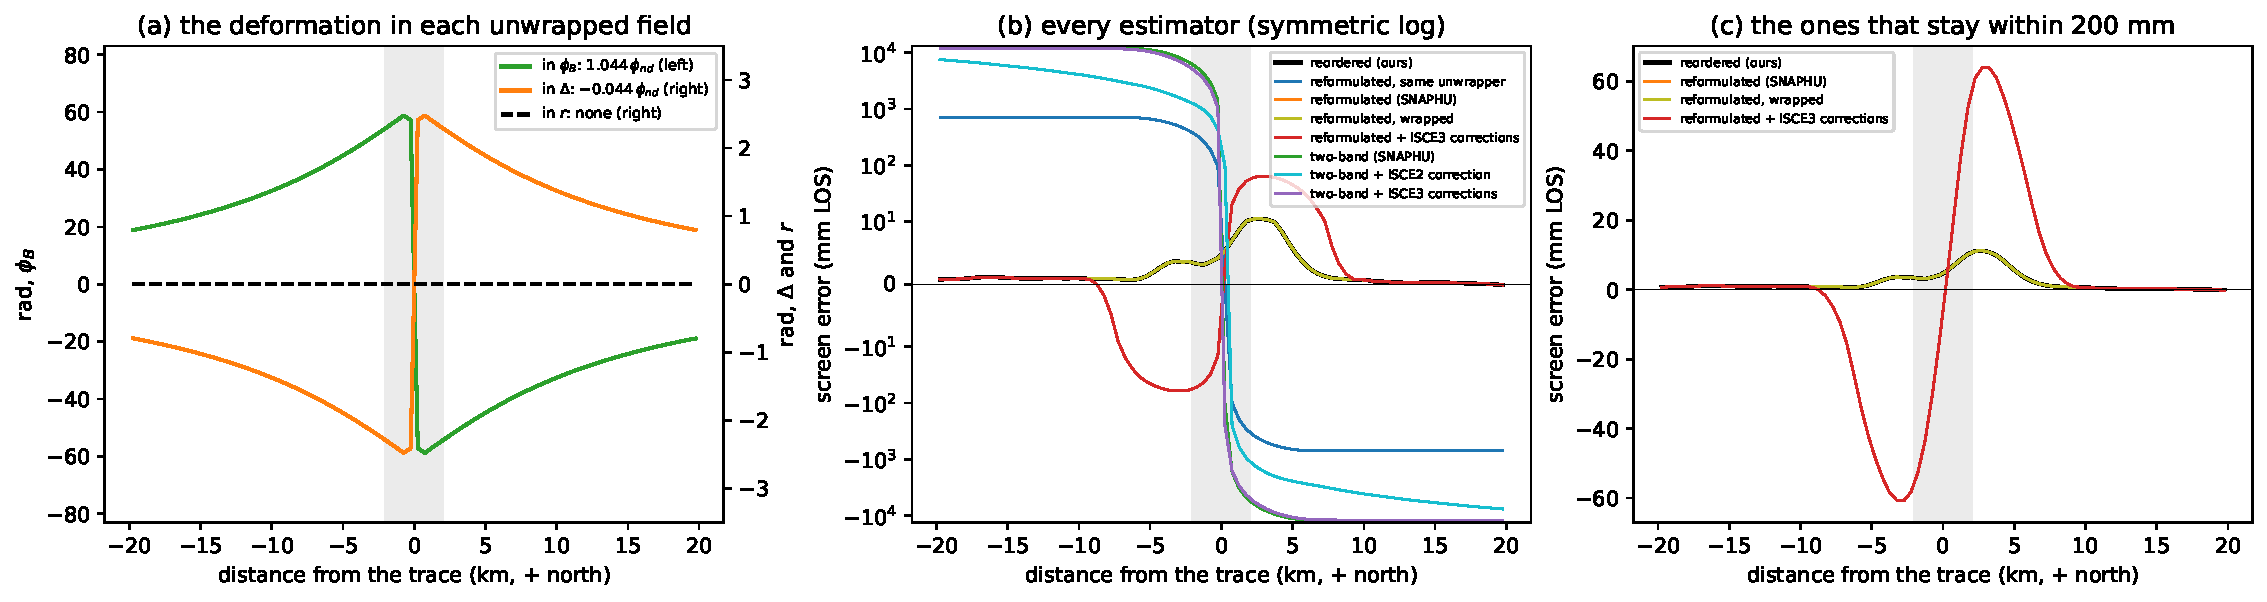
\includegraphics[width=\textwidth]{figures/fig_profiles}
\caption{(a) The deformation each form unwraps, across the through-going 4\,m rupture: all of it in $\phiB$, 4.4\%
in $\Delta$, none in $r$; grey is the excluded fault zone. (b, c) Each estimator's screen error across the trace, as
the median over 0.5\,km bins.}
\label{fig:profiles}
\end{figure}

\begin{figure}[t]
\centering
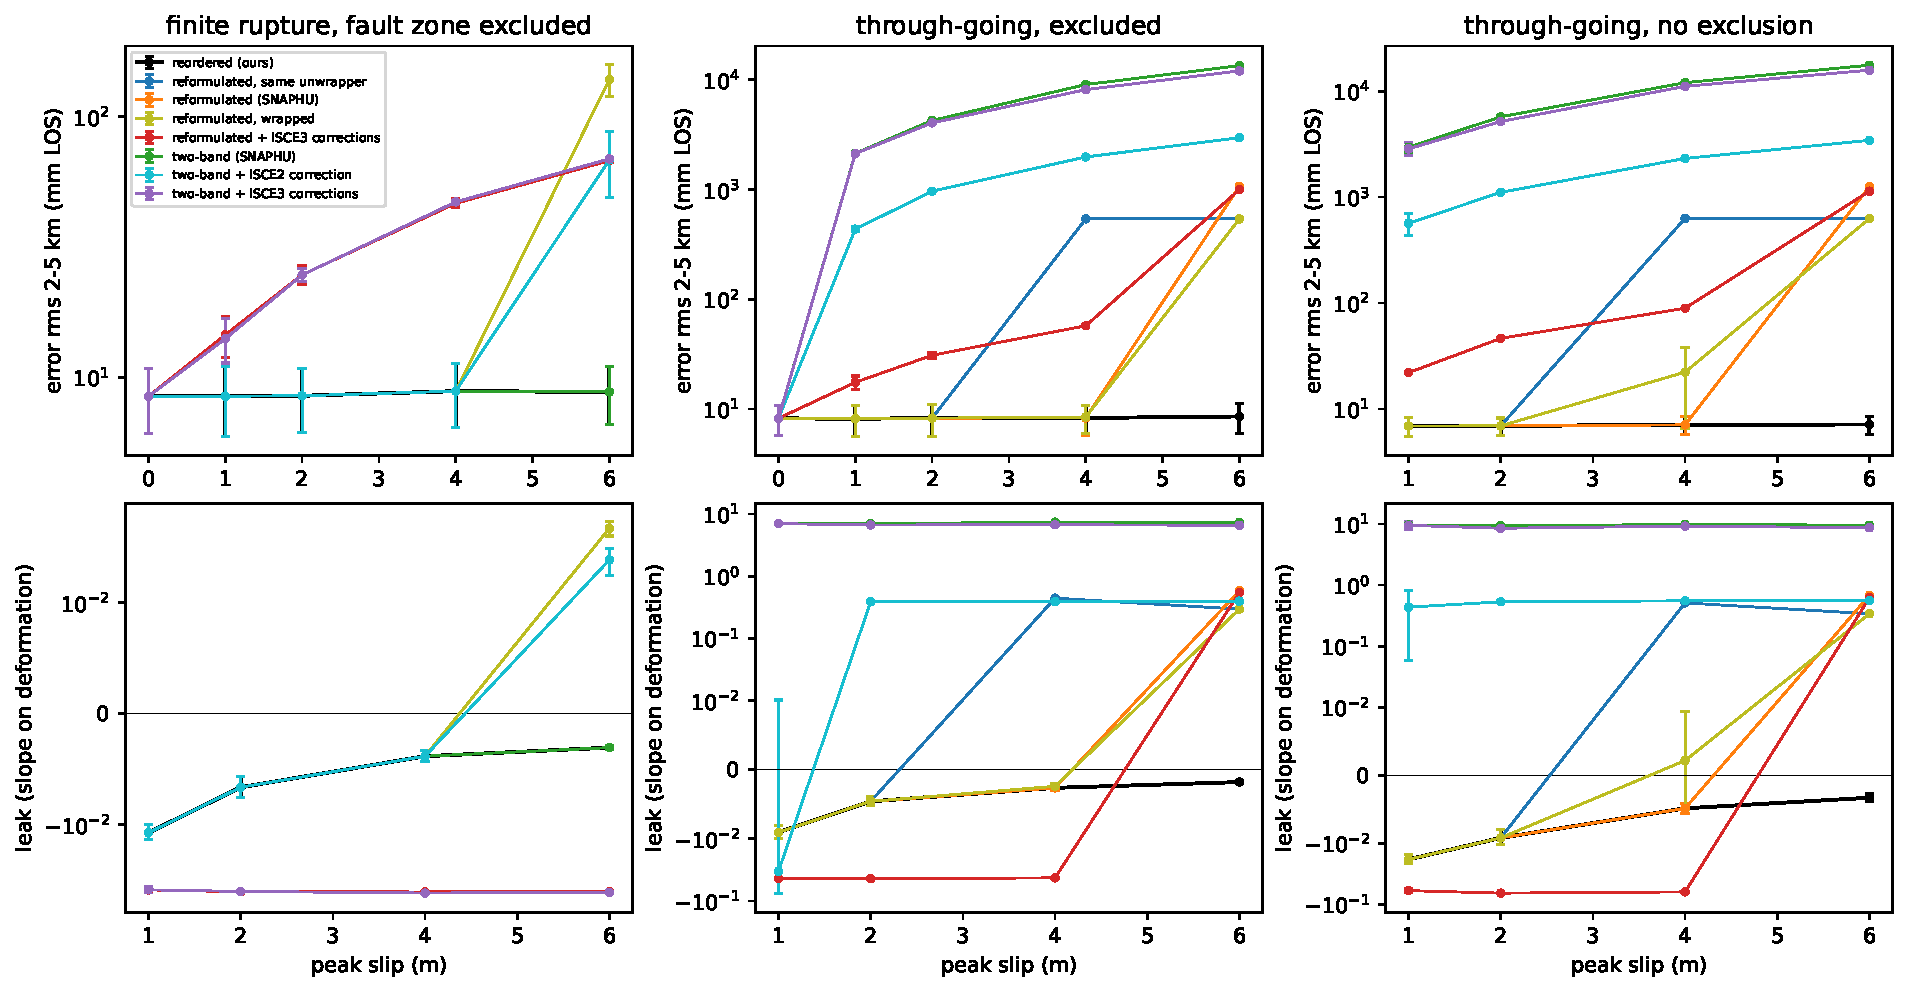
\includegraphics[width=\textwidth]{figures/fig_sweep}
\caption{Error 2--5\,km from the trace and leak against peak slip, mean and spread of three noise realizations. Left:
the rupture ends inside the scene. Middle: it runs through it. Right: as middle, without the fault-zone exclusion.}
\label{fig:sweep}
\end{figure}
